%!TEX root = index.tex
\chapter{State of the art}
\section{Definitions}

Air Traffic Control service (ATC) can be devided into: area control service (ACC), approach control service (APP) and aerodrome control service (TWR) \cite[Chapter 1]{doc4444} The main objective is to prevent collisions between aircraft in air or on land and to expedite the flow of air traffic. \cite[Chapter 2.2]{annex11}
The airspace in which ATC service is provided can be divided into Control area (CTA), Control Zones (CTR) and Controlled aerodromes (TWR). Control area contains airways, terminal control areas and other airspace. It extends upwards from specified altitude. Within CTA, terminal control areas (TMA) are established to help in arrival and departure at some airports.
Control zones are normally situated below CTA and encompass airspace used by flights arriving at and departing from aerodromes. The diameter of CTR is at least 5NM in direction from which airplanes approach. CTR extends from the ground at least to the lower limit of CTA, but may extend further. CTR may include several aerodromes situated close together. \cite[Chapter 2.10]{annex11}

\begin{figure}[h]
    \centering
    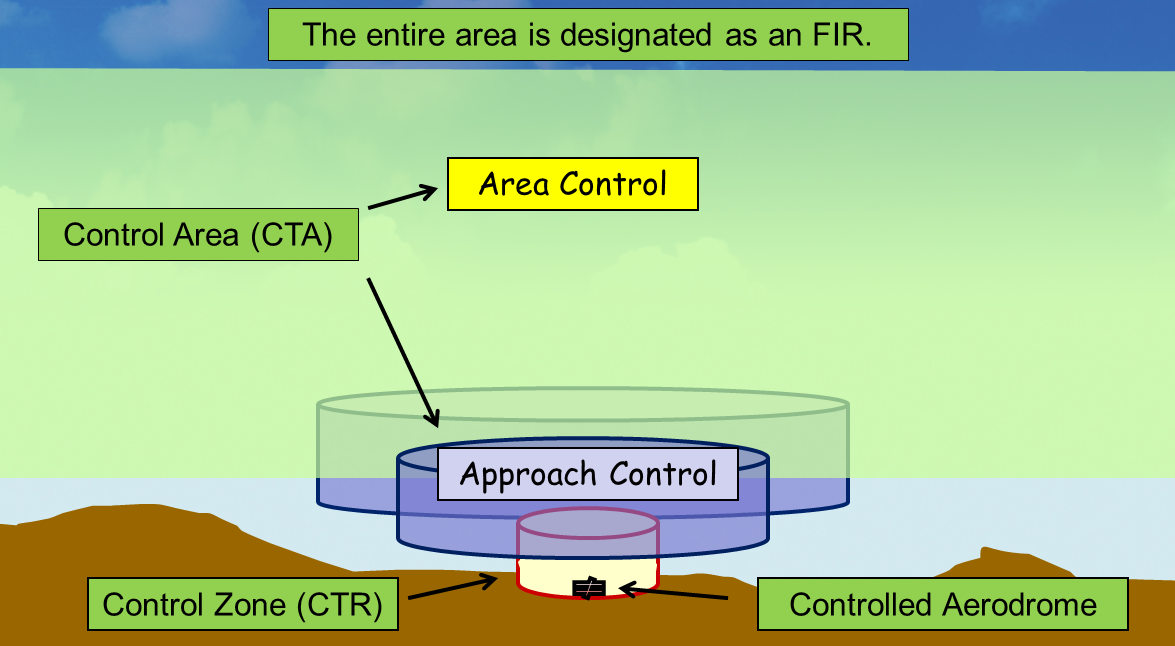
\includegraphics[width=0.8\textwidth]{figures/airspace.png}
    \caption{Airspace - \textcolor{red}{z prezentace 2011 ATM Lesson Plans/ATM 1-1 General Air Traffic Services podle \cite[Chapter 2.5]{annex11} - překreslit!}}
    \label{fig:airspace}
\end{figure}

\begin{figure}[h]
    \centering
    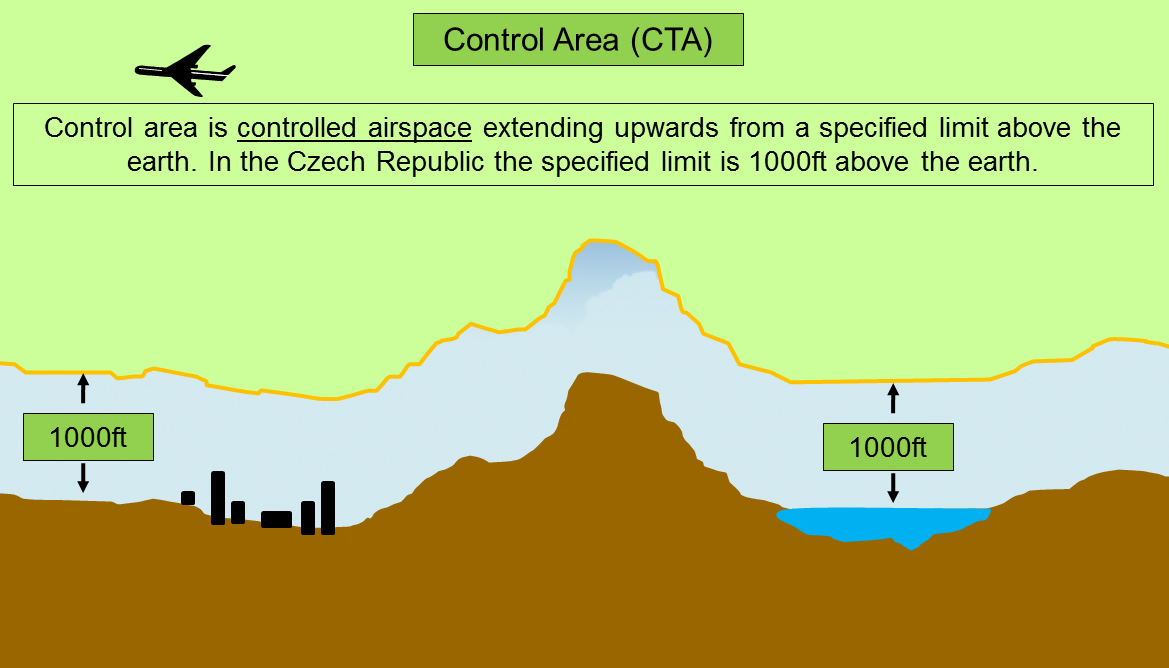
\includegraphics[width=0.8\textwidth]{figures/cta.png}
    \caption{CTA - \textcolor{red}{z prezentace 2011 ATM Lesson Plans/ATM 1-1 General Air Traffic Services podle \cite[Chapter 2.10]{annex11} - překreslit!}}
    \label{fig:cta}
\end{figure}

\begin{figure}[h]
    \centering
    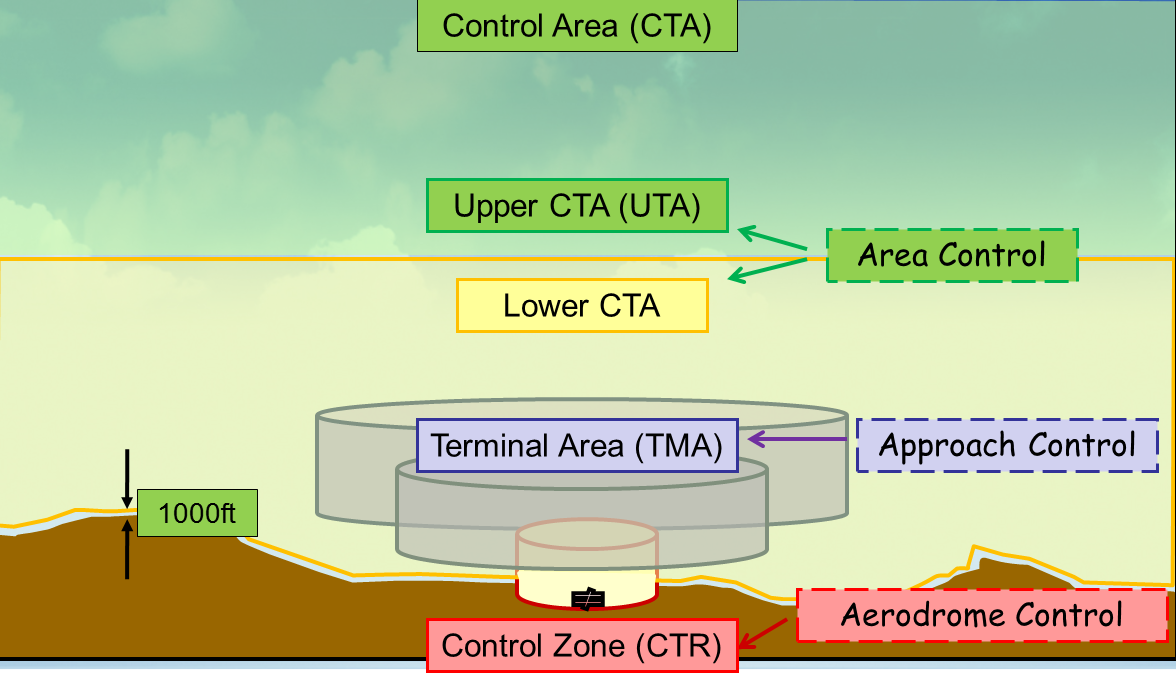
\includegraphics[width=0.8\textwidth]{figures/airspace2.png}
    \caption{Airspace - \textcolor{red}{z prezentace 2011 ATM Lesson Plans/ATM 1-2 General Air Traffic Control Service \cite[Chapter 2.10]{annex11} - překreslit!}}
    \label{fig:airspace2}
\end{figure}

\subsubsection{Area Control Service}
Area Control Service is an ATC service provided by area control centre (ACC) responsible for flights in Control Areas (CTA). Normally ACC is identified by the name of a nearby city, area or landmark. Smaller countries usually have one ACC, but many larger countries are controlled by several of them. ACCs usually control aircrafts in their en-route phase of flight. The ACC may be also responsible for flights to and from smaller aerodromes with no separate approach control service. \cite[Chapter 3.2]{annex11}

\subsubsection{Approach Control Service}
Approach Control Service (APP) is ATC service that is responsible for the part of CTA and CTR required by arriving or departing controlled flights (TMA). The primary functions of APP is sequencing arriving aircrafts and assisting departing aircrafts becoming established on course. The arrival and departure functions can be divided into several positions on busy aerodromes. APP is usually identified by the name of the aerodrome which it is serving, but sometimes it's not colocated with TWR and is at distant ACC location. When no separate ACC exists, approach control service is provided by ACC or TWR. \cite[Chapter 3.2]{annex11}

\subsubsection{Aerodrome Control Service}
Aerodrome control service is provided by a control tower (TWR) and is responsible for aircraft landing and taking off. It's also responsible for VFR flights in the CTR and for preventing collisions between aircrafts on the manoeuvring are of the aerodrome. \cite[Chapter 3.2]{annex11}

\textcolor{red}{z pohledu prostoru/z pohledu kontroly}

\textcolor{red}{v každou chvíli řídí letadlo jeden subjekt a místo a čas předání kontroly je jesně definované - kdy a jak?}

The controlled airspace can furthermore be classified as Class A-G. \cite[\textcolor{red}{kapitola}]{nolan} \textcolor{red}{popis jednotlivých classes podle nolana}

\textcolor{red}{Pro řízení v terminální oblasti nás zajímají všechny druhy řízení/prostoru, Agentfly má zatím jen ACC v CTA?}

\begin{figure}[h]
    \centering
    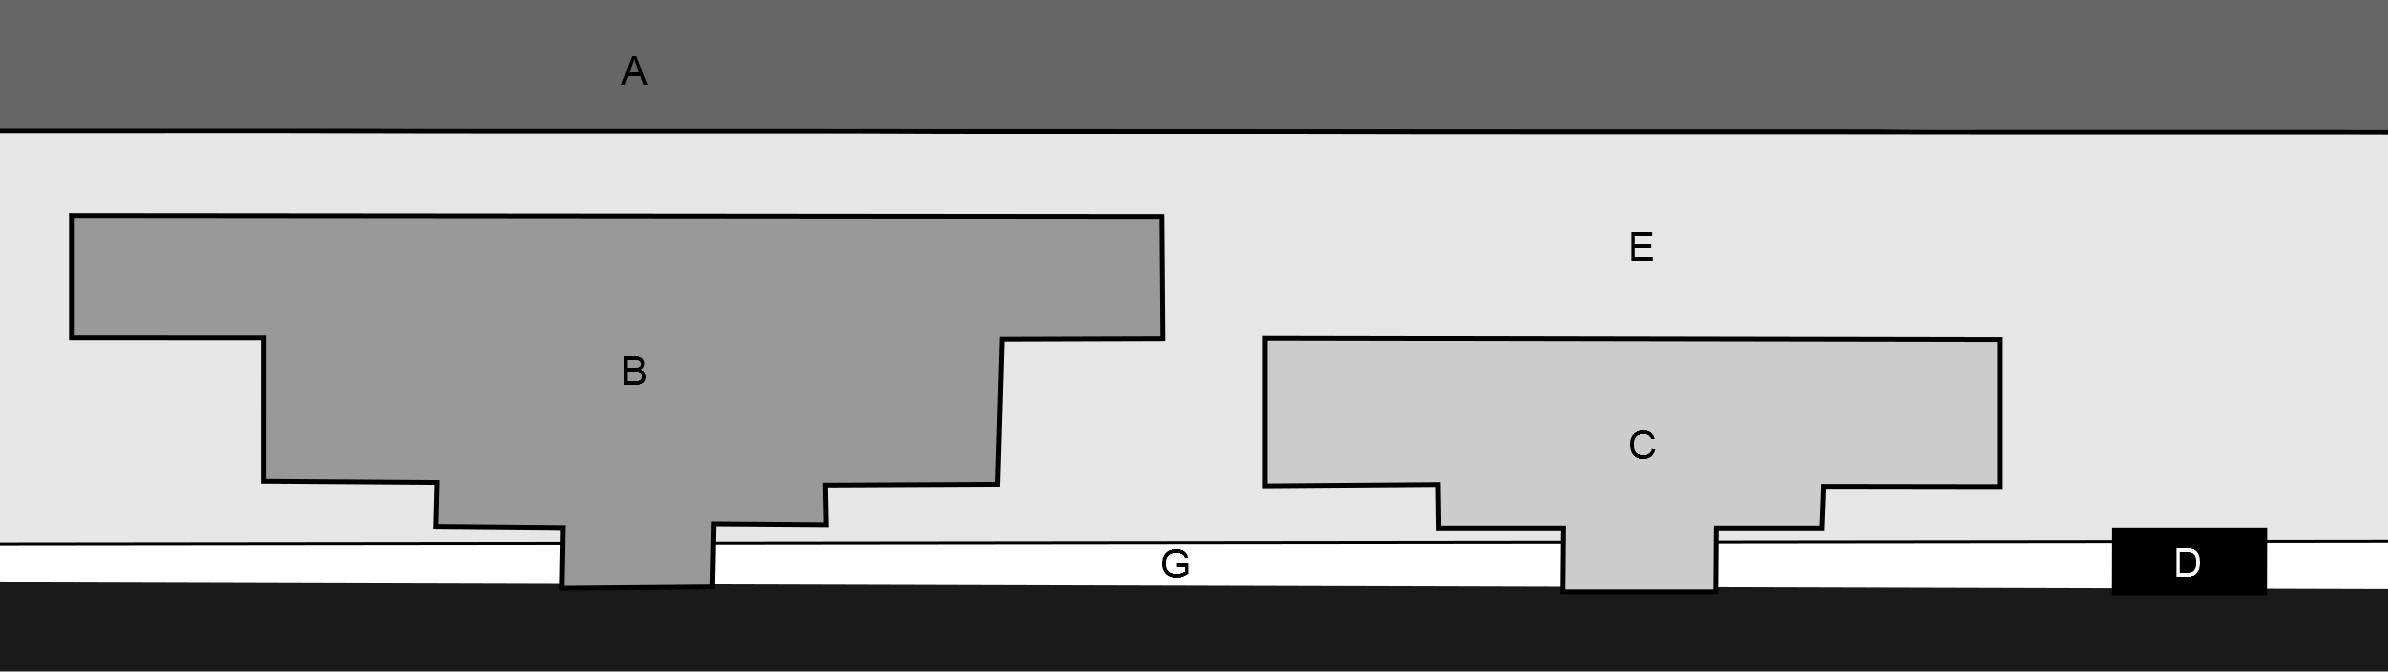
\includegraphics[width=0.8\textwidth]{figures/classes.png}
    \caption{Airspace Classification - \textcolor{red}{z prezentace 2011 ATM Lesson Plans/ATM 1-2 General Air Traffic Control Service \cite {nolan} - překreslit!}}
    \label{fig:classes}
\end{figure}

\textcolor{red}{SID a STAR routy?}

\subsubsection{Airspace Management}
ATM is generic term for any management activity for achieving the most eficient and flexible use of airspace avoiding permanent airspace segregation. \textcolor{red}{zdroj jen z prezentace}
The goals are to improve coordination between civil and military agencies, optimise route network and airspace structure and develop a free route airspace concept.

The concept of Flexible Use of Airspace (FUA) means that airspace should be treated as one continuous space that is being allocated according to user requirements. Any airspace segregation should only be temporary.

\subsubsection{Coordination within ATC}
unit $\leftrightarrow$ unit \\
ACC $\leftrightarrow$ APP \\
APP $\leftrightarrow$ TWR \\
sector $\leftrightarrow$ sector \\
sectors are within units

koordinaci mezi sektory popisuje \cite{doc4444} Doc 4444 Chapter 10
Detailed procedures are often subject to local regulations and rules.

Transferring unit/controller transfers the responsibility to control the aircraft to the accepting unit on point of transfer of control.

The transfer of control can be divided into three stages. First the flight is \bold{notified} to prepare for the transfer. Then the conditions of transfer of control are \bold{negotiated} with the transferring ATC unit and if necessary also with the accepting unit. After the parties \bold{agree}, the control is transferred to the accepting unit. his process can be achieved using automated means (AFTN, RDPS, FDPS, OLDI \textcolor{red}{?}) without using conventional telephone coordination. \textcolor{red}{(Jakože mezi sektory, s letadlem domluva asi pořád probíhá.)} \cite[Chapter 10.1.1]{doc4444}

This means that the flight is at any time under the control of only one ATC unit and can't be transferred from one unit to another without consent of the accepting unit. Also if communication with the aircraft is transwerred to the next unit, that unit cannot change the learance of the aircraft before the point of control transfer.

Doslovně z prezentace:
Control of an aircraft shall be transferred from ACC to APP, and vice versa, at a time or point agreed between the two units. This time or point is normally stated in a LOA.
Except when otherwise specified, APP may issue clearances to any aircraft released to it by ACC without reference to ACC. If an aircraft executes a missed approach, if necessary, ACC shall be informed immediately and subsequent action coordinated. 
After coordination with APP, ACC may release an arriving aircraft directly to TWR if the entire approach will be made under VMC.\cite[Chapter 10.1.3.1]{doc4444}

Doslovně z prezentace:
The take-off time is specified by the ACC when it needs to coordinate the departure with other ACC traffic or provide separation between other departing traffic on the same track. In other cases the APP determines the time of take-off so that the traffic in their AOR is separated. ACC and APP can also specify clearance expiry time if a delayed departure would cause separation problems. The time given by APP must not be later than ACC time. co je AOR?\cite[Chapter 10.1.3.2]{doc4444}

Doslovně z prezentace:
Exchange of movement and control data
APP shall keep ACC advised of data about controlled traffic such as:
RWY in use and type of instrument approach procedure;
lowest available level at the holding fix for use by ACC;
average time or distance intervals between successive arrivals as determined by APP;
revision of EATs as required (5 MIN or greater, or as agreed);
arrival times over holding fix when these vary by 3 MIN or greater from the times estimated by ACC;
flights cancelling IFR, if it will affect holding levels or EATs;
departure times, or if agreed, boundary or specified point times;
information relating to overdue or unreported aircraft; and
missed approach times which may affect ACC.
\cite[Chapter 10.1.3.3]{doc4444}

Doslovně z prezentace:
ACC shall keep APP advised of data about controlled traffic such as:
identification, type and point of departure of arrivals;
ETA and level of arrivals over holding fix or other specified point;
ATA and level of arrivals over holding fix if aircraft is released to APP after arriving over the holding fix;
requested type of instrument approach procedure if different to that specified by APP;
EAT issued;
when required, that an aircraft has been instructed to contact APP;
when required, that an aircraft has been released to APP, including if necessary, the time and conditions of release; and
anticipated delay to departures due to congestion.
ACC shall forward information on arrivals at least 15 MIN before ETA. \cite[Chapter 10.1.3.3]{doc4444}

Doslovně z prezentace:
Division of control
APP shall retain control of arrivals until the aircraft have been transferred to, and are in communication with TWR. Rules for transfer of control of arrivals shall be establish by LOAs or local instructions, considering airspace structure, terrain, MET conditions and ATS facilities available.
APP may authorize TWR to release a departure for take-off subject to the discretion of TWR with respect to arrivals.
TWR shall obtain approval from APP prior to authorizing SVFR flights, when so prescribed in LOAs or local instructions. \cite[Chapter 10.1.4.1]{doc4444}

Doslovně z prezentace:
Exchange of movement and control data
TWR shall keep APP advised of data about controlled traffic such as:
\bitem
\item arrival and departure times;
\item when required, that the first aircraft in the approach sequence is in  	communication with and is sighted by TWR, and that reasonable 	assurance exists that a landing will be accomplished;
\item information relating to overdue or unreported aircraft;
\item information concerning missed approaches; and
\item information concerning aircraft that are essential local traffic to aircraft 	under the control of APP.
\eitem
\cite[Chapter 10.1.4.2]{doc4444}

Doslovně z prezentace:
Transfer of control
For arriving aircraft control shall be transferred from APP to TWR when the aircraft:
\bitem
\item is in the vicinity of the aerodrome, and
	\bitem
	\item it is considered that approach and landing will be completed in visual reference to the ground, or
	\item has reached uninterrupted VMC; or
	\eitem
\item is at a prescribed point or level; or
\item has landed, 
	as specified in LOAs or unit instructions.
\eitem
Transfer of communication to TWR should at a point, level or time that landing clearance, alternative instructions and essential local traffic information can be issued in a timely manner.

For departing aircraft control shall be transferred from TWR to APP:
\bitem
\item when VMC prevail in the vicinity of the aerodrome:
	\bitem
	\item prior to the time the aircraft leaves the vicinity of the aerodrome;
	\item prior to the aircraft entering IMC; or
	\item when the aircraft is at a prescribed point or level, as specified in LOAs or unit instructions; 
	\eitem
\item when IMC prevail at the aerodrome:
	\bitem
	\item immediately after the aircraft is airborne; or
	\item when the aircraft is at a prescribed point or level, as specified in LOAs or unit instructions.
	\eitem
\eitem
\cite[Chapter 4.3.2]{doc4444}

Control shall be transferred from one sector/position to another within the same ATC unit at a point, level or time, as specified in local instructions.
FPL and control information shall be exchanged between control positions within the same unit, in respect of:
  all aircraft for which control will be transferred from one unit to another;
  aircraft operating in such close proximity to an adjacent sector boundary 	that control of traffic in that sector may be affected;
  all aircraft for which control will be transferred from a procedural controller 	to a surveillance controller, as well as other aircraft affected.
These transfer of control and coordination procedures shall conform to agreements applicable to the ATC units.
Even with all the modern electronic equipment and highly developed systems, coordination between controllers within a single sector, or adjoining sectors, if often based on clear, simple conversation. 
This conversation is often conducted in the local native language or, when controllers are busy and occupied with other responsibilities, this communication may be conducted using body language (e.g. raising a hand or nodding the head). 
Such coordination is normally not specified in local rules, and it important that controllers are very careful to ensure there is no misunderstanding between them.
\cite[Chapter 4.3.5, 10.1.5]{doc4444}

ICAO requires that a flight plan (FPL) message containing basic flight plan data is forwarded to the first ACC at least 30 minutes in advance of the flight, and to successive ACCs at least 20 minutes in advance of the flight reaching their area. Normally, due to flow control procedures and general air traffic planning requirements, this minimum is increased to 1 hour or even more, depending on agreements between units. 
If ATC clearances change the route of flight so the aircraft will fly through other ATC areas of responsibility, a current flight plan (CPL) message must be forwarded to those units at least 20 minutes prior to entering their area. Normally, agreements between units will specify an increased time.
An estimate (EST) message shall be forwarded at least 20 minutes prior to a flight entering a unit’s area of responsibility. This message contains the essential control information such as estimate, level and SSR code. The 20 minute time period may be increased or decreased, based on unit requirements and agreements.
\cite[Chapter 11.3,4]{doc4444}

Most common types of ATC coordination:
\bitem
\item current flight plan (20 MIN or more prior to control boundary) 
\item estimate (20 MIN prior to control boundary, or LOAs); 
\item revision (no ICAO defined time, LOAs);
\item approval request (no ICAO defined time, LOAs); and
\item transfer of control.
\eitem

\subsection{Altimetry}
Výška nad mořem/terénem/tlak/potřeba referenční hladiny, závisí na teplotě=tlaku vzduchu

QNE - standardní nastavení - letí se podle flight levelů - výška od referenční hladiny 1013.2 hPa
QNH - letí se podle nadmořské výšky, je to hodnota tlaku na daném místě (typicky letišti) který po zadaání do výškoměru vrací správnou nadmořskou výšku
QFE - výška nad povrchem země v daném místě - typicky u letiště


Transition altitude
The TA is the altitude at or below which the vertical position is expressed in terms of altitudes. The TA is established by the appropriate ATS authority.

Transition level (TL) is flight level just above the TA. Transition layer is the layer between TA and TL. It is prohibited to fly on the level that is in the transition layer.

When the plane is descending the pilot changes from QNE to QNH when passing TL. When climbing pilot changes from QNH to QNE on TA.

Řídící musí včas předat letadlu hodnotu QNH a TL.

\subsection{Separation}
Vertical or horizontal separation shall be provided:

between all flights in Class A and B airspaces;
between IFR flights in Class C, D and E airspaces;
between IFR and VFR flights in Class C airspace;
between IFR and Special VFR flights; and
between Special VFR flights, when so prescribed.
\cite[Chapter 5.2]{doc4444}

Separation should be achieved by one of the following:
\bitem
\item vertiacal - planes are assigned different cruising levels
\item horizontal
	\bitem
	\item longitudinal - interval between planes flying on the same (converging, reciprocal) is maintained
	\item lateral - planes fly on different routes
	\eitem
\item composite - combination of the above
\eitem
\cite[Chapter 3.3]{doc4444}

\subsubsection{Vertical}
Reduced vertical separation minima
doslovně
Minima
Within RVSM airspace 
1000ft between FL290 and FL410 inclusive, and
2000ft above this level

Within other airspace
1000ft below FL290, and
2000ft above FL290

IFR flight levely vyhrazené pro jednotlivé směry: liché desítky na východ (0$^{\circ}$-179$^{\circ}$), sudé na západ(180$^{\circ}$-359$^{\circ}$)

VFR flight levely končí pětkou

\subsubsection{Longitudinal}
15/10/5 minut separace nad stejným bodem podle typu situace 
\cite[Chapter 5.4.2.2]{doc4444}

\subsection{Wake Turbulence Separation}
Its the air vortex formed behind every aircraft. It's size and strength depends on the parameters of the aircraft (size, mass, speed, wing configuration...). It's not visible and can be hazardous for the following aircraft.

Special attention is needed in light wind conditions, because the turbulence can remain for a considerable time and may drift to parallel runway or sink to the path of following aircraft.

\subsubsection{Minima (for procedural control?)}
For arriving MEDIUM aircraft after HEAVY: 2 minutes. LIGHT after HEAVY 3 minutes. \cite[Chapter 5.8.2]{doc4444}
For departing LIGHT or MEDIUM aircraft after HEAVY: 2 minutes. LIGHT after MEDIUM 2 minutes. \cite[Chapter 5.8.3]{doc4444}
A DALŠÍ VARIANTY... viz prezentace

\subsubsection{Minima (for surveillance control?)}
\bitem
\item Heavy - 136 tonne or more
\item Medium - 7-136 tonne
\item Light - 7 tonne or less
\eitem
For both arrival and departure of planes provided with surveillance service: (also enroute at the same altitude or less than 1000ft below or parallel runway separated by less than 2500ft)
\bitem
\item H after H: 4NM
\item M after H: 5NM
\item L after H: 6NM
\item L after M: 5NM
\eitem
\cite[Chapter 8.7.3]{doc4444}

\subsection{Holding}
Holding procedure is a predefined manouvre that keeps the aircraft in predetermined airspace while waiting for clearance. The procedure is the same for VFR and IFR flights.
Expected Approach Time (EAT) is the time when arriving aircraft leaves the holding fix in order to complete its approach for landing. Holding fix is a geographical location that serves as a reference point for holding procedure.
\cite[Chapter 6.5.8]{doc4444}

Reasons for holding can be traffic congestion, delays at destination airport or aircraft problems.

\begin{figure}[h]
    \centering
    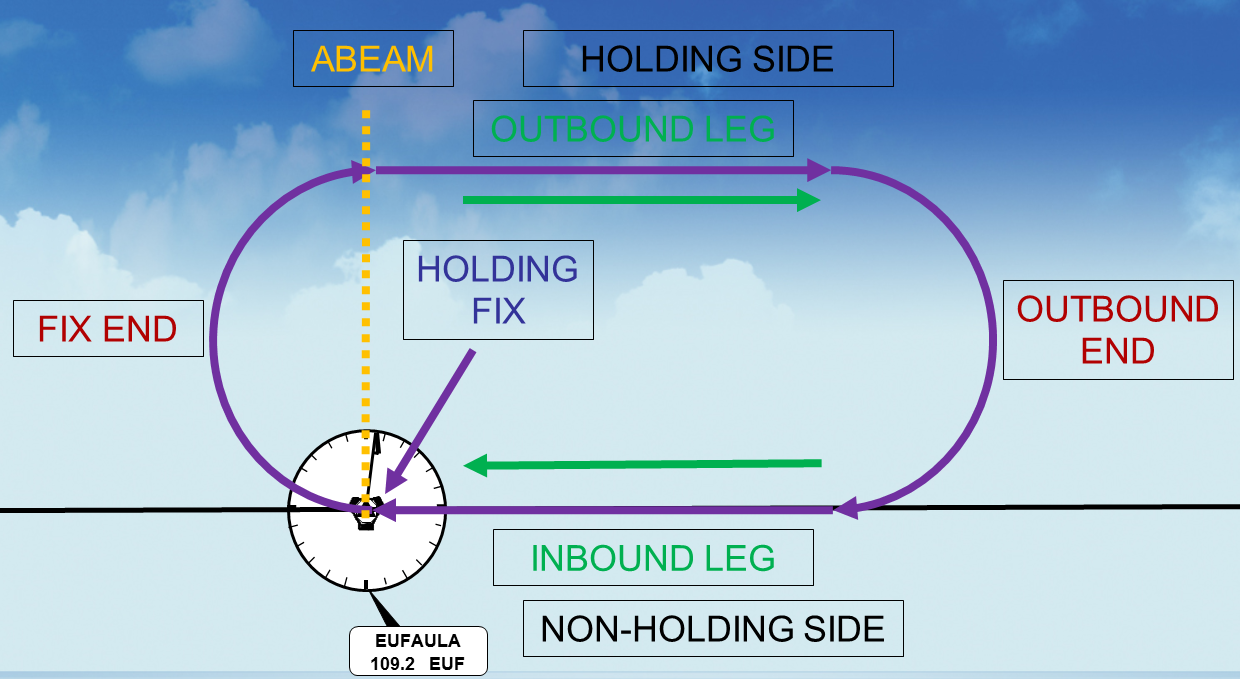
\includegraphics[width=0.8\textwidth]{figures/holding.png}
    \caption{Holding pattern - \textcolor{red}{z prezentace 2011 ATM Lesson Plans/ATM 18 Holding - překreslit!}}
    \label{fig:classes}
\end{figure}
\begin{figure}[h]
    \centering
    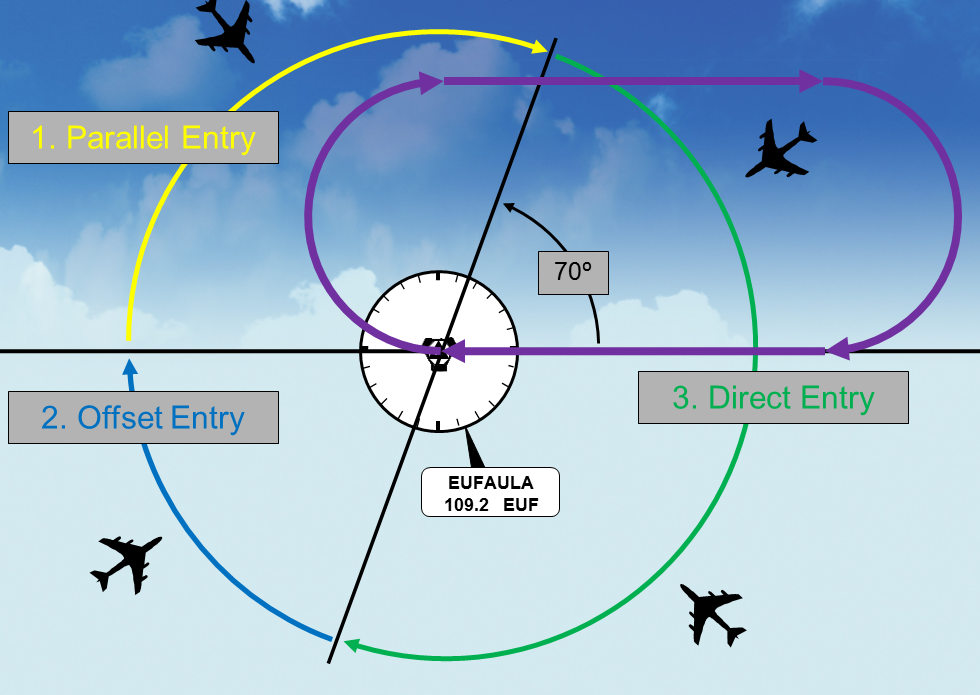
\includegraphics[width=0.8\textwidth]{figures/holding-entry.png}
    \caption{Entry procedures - \textcolor{red}{z prezentace 2011 ATM Lesson Plans/ATM 18 Holding - překreslit!}}
    \label{fig:classes}
\end{figure}
Doplnit popis jednotlivých entry procedures!

If the delay is expected, the aircraft should be notified as soon as possible and if practical advised to reduce speed in order to absorb the delay. The ACC is normally responsible for clearing the aircraft to the holding fix including the instruction for the holding procedure itself and EAT.\\
The holding procedure (including the pattern etc.) is normally published beforehand. Otherwise ATC shall specify the details of the procedure. Normally the first arriving aircraft is at the lovest level and the following aircrafts at successively higher levels. Turbojet aircrafts can be held at higher levels in order to conserve fuel, but ther order must be retained.\\
Vertical separation is mantained amongst the aircrafts in the holding sequence. Vertical separation must be applied whenever other aircraft is within 5 minutes of the holding area.\cite[Chapter 6.5.5]{doc4444}

The EAT should be established for aircrafts expected to be delayed for 10 minutes or more and transmitted to the aircraft as soon as practicable. It should be retransmitted if the updated EAT differs from the previous time by 5 minutes or more.\cite[Chapter 6.5.7]{doc4444}

\textcolor{red}{konec 19}